\documentclass[a4paper,10pt]{article}
\usepackage[utf8]{inputenc}
\usepackage[frenchkw]{algorithm2e}
\usepackage[francais]{babel}
\usepackage{graphicx}
\usepackage{amsfonts}
\usepackage{amsmath}
\usepackage{color}
\usepackage{float} 
\usepackage{float} 
\usepackage{listings}

\lstset{language={Python}} 
 
%pour gerer les marges 
\newenvironment{changemargin}[2]{\begin{list}{}{% 
\setlength{\topsep}{0pt}% 
\setlength{\leftmargin}{0pt}% 
\setlength{\rightmargin}{0pt}% 
\setlength{\listparindent}{\parindent}% 
\setlength{\itemindent}{\parindent}% 
\setlength{\parsep}{0pt plus 1pt}% 
\addtolength{\leftmargin}{#1}% 
\addtolength{\rightmargin}{#2}% 
}\item }{\end{list}}

%opening
\title{}
\author{}

%Il reste à faire:
%raccourcir de 5000 carctères
%Juliette :

%seulement entre 1 et 40 notes" : le graphique montre un maximum de note à 25. (voir commentaires de Emiya)
% verifier le titre pour un de tes graphiques : "Notes rangées en fonction du nombre de fois qu'ont été notés les films qu'elles notent"
% améliorer les titres que j'ai mis à tes graphiques si tu penses que c nécessaire de le faire

\begin{document}

\renewcommand{\thepage}

\begin{titlepage}


\includegraphics[width=4cm]{image1.png}
\hfill

\includegraphics[width=4cm]{centrale_logo.jpg} 
\color{white}{ .}
\vspace{4cm}
 \color{black}
	\begin{center}
		\textsc{\Huge \underline{Recommandation de films} }\\
		[1.5cm]
		\color{black}
		\textsc{\normalsize  AUGUSTONI Guillaume, AMRAM Yassine, PHILIBERT Juliette, GIRAUDO Anthony}\\
		[0.75cm]
		\textbf{\small Licence 1ère année - Mathématiques, Physique, Chimie, Informatique}\\
		[0.3cm]	
		\textrm{\small 2016-2017}\\
		[0,75cm]
		\textbf{\normalsize Encadrant de projet: } 
		\textsc{\normalsize Emiya Valentin}\\
	\end{center}
\end{titlepage}

%page de garde :
\newpage
\strut
\newpage

%remerciements :

\section*{Remerciements}

Nous remercions notre encadrant de projet, Valentin Emiya qui nous a guidé et soutenu tout au long de ce projet. \\

Nous remercions également Victoria Paolantoni qui nous a débloqué pour la rédaction de l'une des preuves.\\

Enfin, nous remercions toutes les personnes ayant participé à la relecture de ce rapport.
\newpage

%Sommaire :

\renewcommand{\contentsname}{Sommaire}
\tableofcontents
\newpage

%commencer la numérotation des pages:
\renewcommand{\thepage}{\arabic{page}}
\setcounter{page}{1}

\section*{Introduction}

A l’ère du numérique, la collecte de données d’une multitude d’utilisateurs peut devenir très intéressante pour leur faire des suggestions 
personnalisées de tout type. C’est une chose que l’on rencontre souvent : recommandations d’amis sur Facebook, suggestions d’achats sur Internet, etc.
Nous avons choisi de nous intéresser à la recommandation automatique de films.
Mais comment recommander à un utilisateur un film qu’il aimera ? Beaucoup de critères peuvent entrer en compte : 
le genre du film, le jeu des acteurs, la date du film, ou tout simplement sa bonne qualité … Tout cela est très subjectif \! \\


Nous en arrivons à la problématique suivante : Comment concevoir un programme informatique permettant une recommandation personnalisée pertinente ?
En se limitant à un certain nombre de films, la méthode proposée lors de ce projet consiste à estimer les notes que mettrait l’utilisateur aux films qu'il n'a pas vu.
Nous pouvons ainsi trouver les films les plus en accord avec ses goûts en regardant les plus hautes prédictions de note.\\
Pour ce rapport, dans un premier temps nous introduirons le sujet en expliquant notre approche du problème.
Puis, nous verrons sur quel modèle mathématique nous nous sommes appuyés pour écrire notre algorithme, et nous finirons par expliquer comment marche notre algorithme et comment l’optimiser.

\newpage

\section{Qu'est ce qu'un système de recommandation?}

\subsection{Notre approche}

Le but de notre projet est de pouvoir recommander un film ou plusieurs à n'importe quel utilisateur. 
Pour cela, nous devons savoir à quel point un utilisateur va aimer tel ou tel film pour le lui recommander ou pas. Ce qui parait alors pertinent est d'estimer pour chaque film une note que lui donnerait l'utilisateur s'il le voyait. 
Nous pourrions ainsi recommander le film ayant la meilleur note prédite.
Notre objectif est alors de trouver un modèle mathématique permettant de déterminer la note que mettrait un utilisateur à n'importe quel film qu'il n'a pas vu. Cependant il nous faut nous appuyer sur quelque chose. Pour commencer à travailler, il faut déjà connaître certaines informations : nous travaillerons avec des notes de films données par un certain nombre d'utilisateurs.

\subsection{Première difficulté : les données}
\subsubsection{Extraction de données}

Le besoin d'avoir des données nous guide vers une grande base de données`` movielens.org '' qui est un site communautaire de recommandation de films où les utilisateurs du site notent des films de 0 à 5.
Plusieurs jeux de données y sont disponibles. 
Nous choisissons de travailler avec des notes données par 670 utilisateurs à 9125 films.
Par la suite nous nous référerons au nombre d'utilisateurs par $n_u$ et au nombre de films par $n_f$.
Nous extrayons alors 2 fichiers : l’un contenant les $n_f$ films dans un tableau avec leurs titres et un numéro d'identification attribué, 
l’autre avec les notes des utilisateurs eux aussi numérotés par des identifiants.
Ce dernier fichier est un tableau avec $n_u$ lignes du type : identifiant de l’utilisateur, id du film qu’il a noté, note. 
Ces 2 fichiers étant peu pratiques pour manipuler leurs données,  
nous créons une fonction tableau\_des\_notes() qui retourne un tableau, une matrice de dimensions $n_u * n_f$ qui contient les notes données par les utilisateurs, en ligne, aux films, en colonne. Seulement, aucun utilisateur n'a noté tous les films : il y a des cases vides dans notre tableau. Nous insérons alors dans ces cases des `` NaN ''(Not a Number), type de donnée facile à traiter dans notre programme.
La matrice des notes est appelée Y.

\begin{figure}[H]
  \centering
  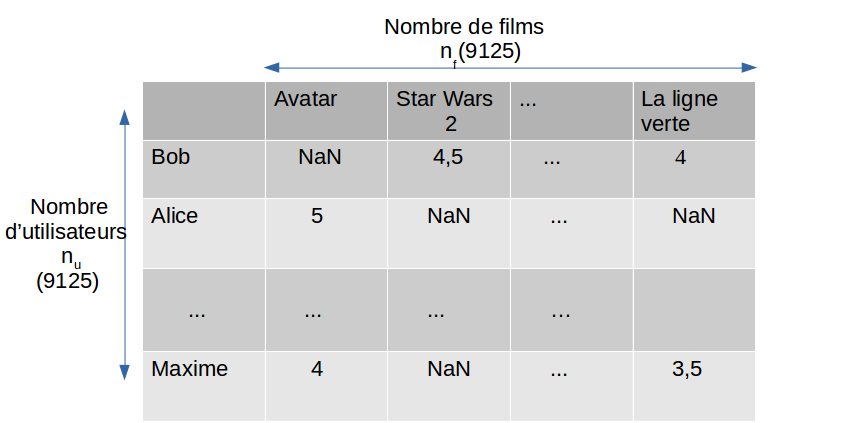
\includegraphics[scale=0.4]{Ynew.png}
  \caption{Tableau des notes Y}
\end{figure}

\subsubsection{Analyse des données}

Nous créons ensuite deux fonctions permettant de faire des statistiques sur nos données : l’une permettant de compter combien de films chaque utilisateur a vu, et l’autre comptant le nombre de notes attribuées pour chaque film. De ces fonctions, nous tirons des graphiques nous permettant d'avoir une idée plus précise de nos données.\\
%là y a un soucis par rapport au graphique 
Nous remarquons alors que plus de 90 \% des films possèdent entre 1 et 40 notes, et que le plus souvent un film a 2 notes. Le film auquel a été attribué le plus de notes a 339 notes.

\begin{figure}[H]
  \centering
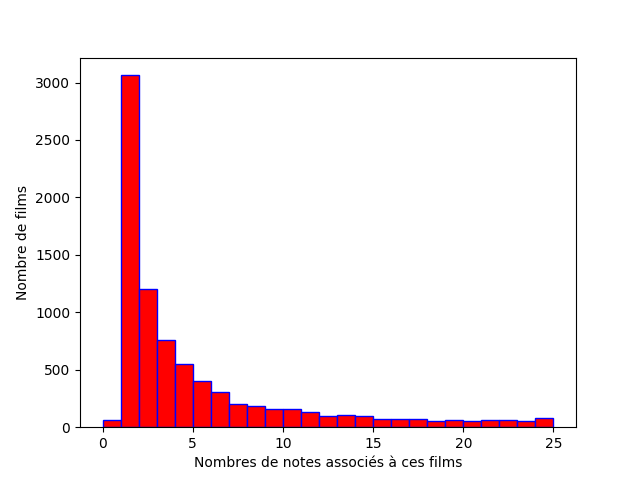
\includegraphics[scale=0.5]{hist2.png}
\caption{Films triés en fonction du nombre de fois qu'ils ont été notés}
\end{figure}

Dans l’autre sens, nous voyons aussi que chaque utilisateur a noté 148 films en moyenne.

\begin{figure}[H]
  \centering
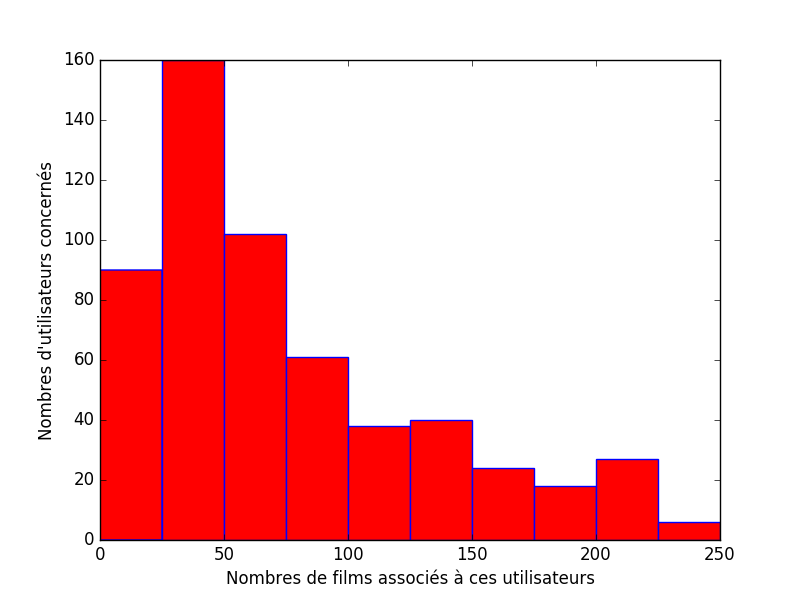
\includegraphics[scale=0.5]{hist1.png}
\caption{Notes rangées en fonction du nombre de fois qu'ont été notés les films qu'elles notent}
\end{figure}

De plus, notre tableau présente 98,4 \% de NaN. Soit plus de 6 millions de notes à prédire !

Notre but devient de compléter ces trous, de prédire les notes que nous ne connaissons pas. Alors nous pourrons, en réutilisant la même méthode, pour n'importe quel personne ayant noté quelques films deviner les notes qu'elle mettra aux films qu'il n'a pas encore vu.

\section{Modélisation du problème}

Nous nous posons maintenant la question de comment nous y prendre pour prédire des notes ?
Notre seule ressource est la matrice Y non pleine. Sur quel modèle s'appuyer pour la compléter ?
C'est ce que nous allons étudier dans cette partie.

\subsection{Factorisation de matrices}

Toutes les notations utilisés sont précisés en \ref{notations}.\\

Posons $Y_f$ la matrice Y complétée qui contient toutes les prédictions, exactes, des notes qui nous manquent. C'est la matrice à laquelle nous voulons aboutir, celle que nous devons deviner. Voici notre méthode.\\ 
 
Nous supposons que nous sommes capable de déterminer à partir de Y deux matrices X et $\Theta$ telles que $\Theta X^T = Y_f$ avec $\Theta$ une matrice de dimensions $n_u * n$ et X une matrice de dimensions $n_f * n$. $n \in \mathbb{N}^*$ est quelconque, nous verrons par la suite que nous pouvons le fixer comme bon nous semble.\\ 
Notre hypothèse sur l'interprétation de $\Theta$ et X ? Ce qui nous fait supposer leur existence ? Nous allons éclairer ce point tout de suite par des explications plus précises.\\

Le paragraphe qui suit est la description de nos suppositions sur l'interprétation que nous pouvons faire à propos de n, $\Theta$ et X. Après chaque verbe au conditionnel il est sous-entendu "d'après notre hypothèse".\\
Parlons un peu du nombre n. Ce dernier serait en fait un nombre de caractéristiques quelconques, qui nous sont inconnues et qui peuvent bien décrire nos films : si nous pensons qu'ils peuvent être décrits efficacement par 10 caractéristiques, nous choisissons de trouver $\Theta$ et X avec $n = 10$. 
Une caractéristique peut être n'importe quoi, du taux d'action au taux de blondeur des cheveux de l'actrice principale. Pour l'instant admettons seulement que ces n caractéristiques peuvent exister. Nous les numérotons de 1 à n, puis nous verrons comment elles sont déterminées dans une autre partie.\\
Décrivons X. Nous avons déjà dit que cette matrice possède $n_f$ lignes. Chaque ligne caractériserait un film. Ainsi $\forall j \in \{1, 2, ..., n_f\}$ le film j serait décrit par $x_j$ de dimensions $1 * n$. Comment ? En fait $\forall k \in \{1, 2, ..., n\}$ $x_{j,k}$ correspondrait à un taux de correspondance entre le film j et la k-ième caractéristique. Si la k-ième caractéristique est l'action et si le film j est un film d'action tandis que le film j' ($j' \in \{1, 2, ..., n_f\}$) est un film romantique sans action alors $x_{j,k}$ sera un réel supérieur à $x_{j',k}$.\\
Décrivons maintenant $\Theta$. $\forall i \in \{1, 2, ..., n_u\}$ $\theta_{i}$ représenterait les goûts de l'utilisateur i. $\forall k \in \{1, 2, ..., n\}$ $\theta_{i,k}$ serait un taux d'appréciation de la caractéristique k pour l'utilisateur i.\\
Ainsi seraient les deux matrices auxquelles nous voulons aboutir.\\

Voyons maintenant voir en quoi le produit $\Theta X^T$ peut valoir $Y_f$. D'après le produit matriciel, $\forall i \in \{1, 2, ..., n_u\}$ et $\forall j \in \{1, 2, ..., n_f\}$ on a $(y_{f})_{i,j} = theta_{i}(x_{j})^{T}$ : la note que l'utilisateur i a donné ou donnera au film j dépend des caractéristiques du film et du profil de l'utilisateur. Et nous avons :
\[(y_{f})_{i,j} = \sum_{k = 1}^{n} \theta_{i,k} * x_{j,k}\]
Ce qui semble logique : la note est une combinaison linéaire des taux de caractéristiques du film avec des coefficient qui sont plus ou moins élevé suivant le goût de l'utilisateur pour la caractéristique concernée.

\subsection{Fonction de coût}

Nous avons supposé que $\Theta$ et X existent, cependant il est très peu probable que ce soit le cas : nous pouvons arriver à deux matrices avec les dimensions voulues mais avec au mieux $\Theta X^T \approx Y_f$. Notre problème devient alors la minimisation de l'écart entre les notes de $\Theta X^T$ et celles de $Y_f$. Mais nous ne connaissons que quelques notes de $Y_f$ : les notes déjà données par les utilisateurs, celles de Y. Ce qui nous amène à introduire une fonction qui estime un écart entre les notes de $\Theta X^T$ et de Y :
\begin{align*}
J\colon{\cal M}_{n_u, n} \times {\cal M}_{n_f, n} &\longrightarrow \mathbb{R}^+\\
(\Theta, X)&\longmapsto \frac{1}{2}\sum_{\substack{i,j \\ y_{i,j} \ne NaN}}(\theta_{i}(x_{j})^{T}-y_{i,j})^{2}
\end{align*}
Nous appelons J fonction de coût, c'est la fonction à minimiser : il faut trouver $\Theta$ et X tels que J(X, $\Theta$) soit le plus bas possible. Ce X et ce $\Theta$ seront ceux qui représenteront nos données le mieux possible.

\section{Implémentation de l'algorithme}
\subsection{Minimiser une fonction ? La descente du gradient}

Nous utilisons un algorithme appelé descente du gradient pour minimiser J. Pour illustrer cet algorithme nous allons l'appliquer à une fonction qui dépend de deux variables : soit
\begin{align*}
f\colon \mathbb{R}^2&\longrightarrow f(\mathbb{R}^2)\\
(x_1, x_2)&\longmapsto f(x_1, x_2)
\end{align*}
Soit $(x_1, x_2) \in \mathbb{R}^2$. Nous avons une variation infinitésimale de f, $df = \frac{\partial f}{\partial x_{1}}d x_{1} + \frac{\partial f}{\partial x_{2}}dx_{2}$ avec $dx_1$ et $dx_2$ respectivement une variation infinitésimale de $x_1$ et une de $x_2$. 
Soit $(\alpha_{x_1}, \alpha_{x_2}) \in (\mathbb{R}^{+*})^2$. 
 Posons $\Delta x_{1} = -\alpha_{x_1} \frac{\partial f}{\partial x_{1}}$
 et $\Delta x_{2} = -\alpha_{x_2} \frac{\partial f}{\partial x_{2}}$. Soit $\Delta f = f(x_1 + \Delta x_1, x_2 + \Delta x_2) - f(x_1, x_2)$. $\Delta f$ est la variation de f lorsque $x_1$ varie de $\Delta x_1$ et $x_2$ varie de $\Delta x_2$. 
En faisant l'approximation $\Delta f = \frac{\partial f}{\partial x_{1}}\Delta  x_{1} + \frac{\partial f}{\partial x_{2}}\Delta x_{2}$ nous obtenons $\Delta f = -\alpha_{x_1} (\frac{\partial f}{\partial x_{1}}(x_1, x_2))^{2} - \alpha_{x_2} (\frac{\partial f}{\partial x_{2}}(x_1, x_2))^{2} < 0$. Ainsi, dans
 les limites de l'approximation faite au dessus, à chaque fois que nous modifions les $x_{k}$ de $- \alpha_{x_k} \frac{\partial f}{\partial x_{k}}(x_1, x_2)$
 nous avons une diminution de la valeur de $f(x_1, x_2)$. Et nous admettons que modifier un certain nombre de fois les $x_i$ de la sorte va faire converger la valeur $f(x_1, x_2)$ vers un minimum si la fonction est convexe sur l'intervalle dans lequel nous modifions les $x_i$.\\

C'est le principe de la descente du gradient et nous obtenons l'algorithme suivant pour minimiser f :
\begin{algorithm}
\caption{Descente du gradient sur f}
\Entree{$\alpha_{x_1}, \alpha_{x_2}$, f}
\Res{$x_1$ et $x_2$ tels que $f(x_1, x_2)$ soit un minimum}
\BlankLine
Affecter à $x_1$ une valeur aléatoire\;
Affecter à $x_2$ une valeur aléatoire\;
\Repeter{convergence de la valeur $f(x_1, x_2)$}{Affecter à $(x_1, x_2)$ la valeur ($x_1 - \alpha_{x_1} \frac{\partial f}{\partial x_{1}}(x_1, x_2), x_2 - \alpha_{x_2} \frac{\partial f}{\partial x_{2}}(x_1, x_2))$\;}
\BlankLine
\end{algorithm}

\noindent Une partie de cet algorithme est répété un certain nombre de fois : nous l'appelons "étape du gradient" ou parfois simplement "étape".\\
Remarquons que $x_1$ et $x_2$ sont fixés aléatoirement : leur valeur de départ peut être quelconque, l'algorithme minimisera quand même f.\\
Notons que $\alpha_{x_1}$ et $\alpha_{x_2}$ sont appelés taux d'apprentissage.
Chose importante, les approximations utilisées ne fonctionnent qu'avec des valeurs assez petite de $\Delta x_1$ et $\Delta x_2$. Il faut donc choisir des taux d'apprentissage eux aussi petits pour que la descente du gradient puisse fonctionner. Mais choisir des taux d'apprentissage trop petits modifierait trop peu les $x_i$ à chaque étape : il faudrait alors un très grand nombre d'étape pour arriver à un minimum de $f$.\\

Depuis le début nous parlons d'un minimum et pas du minimum. En fait la descente du gradient permet d'arriver à un minimum local d'une fonction. Pour minimiser J, nous avons décidé de nous contenter d'un minimum.

\subsection{Minimiser J}

Nous voulons maintenant appliquer le même raisonnement sur $J$ pour modifier X et $\Theta$, initialement pris aléatoirement, un certain nombre de fois jusqu'à arriver à une valeur de $J(X, \Theta)$ assez faible. Voyons voir comment s'y prendre.\\

La différence avec la partie précédente, c'est que nous parlons de matrices. Mais chacun des coefficients de ces matrice peut être considéré comme une variable. Nous pouvons alors utiliser la descente du gradient pour J en considérant qu'il s'agit d'une fonction à $n_u * n + n_f * n$ variables. Or utiliser la descente du gradient comme ceci est beaucoup trop long : 30 secondes par étape avec $n = 10$ sachant qu'il nous faut plus de 500 étapes pour arriver à un résultat correct.\\

Or, nous remarquons que faire ce qui est décrit au dessus revient à faire à chaque étape :

\begin{algorithm}
\Entree{X, $\Theta$, $\alpha_X$, $\alpha_{\Theta}$, J}  
\Res{X et $\Theta$ tels que J(X, $\Theta$) se soit rapproché du minimum de J}
\BlankLine
\textbf{Simultanément:}\\
\indent \PourTous{j $\in$ \{1, 2, ..., $n_f$\}}{Affecter à $x_{j}$ la valeur $x_{j}-\alpha_X (\nabla_{(x_{j})^T}J(X, \Theta))^T$\;}
\indent \PourTous{i $\in$ \{1, 2, ..., $n_u$\}}{Affecter à $\Theta_{i}$ la valeur $\theta_{i} - \alpha_{\Theta} (\nabla_{(\theta_{i})^T}J(X, \Theta))^T$\;}
\caption{Étape de la descente du gradient}
\end{algorithm}

\noindent Cela en considérant une matrice colonne comme un vecteur pour calculer le gradient et en considérant le gradient comme une matrice colonne (voir \ref{notations}).\\
Il faudrait maintenant être capable de calculer rapidement $\nabla_{(x_{j})^T}J(X, \Theta)$ $\forall j \in \{1, 2, ..., n_f\}$ et $\nabla_{(\theta_{i})^T} J(X, \Theta)$ $\forall i \in \{1, 2, ..., n_u\}$.
Nous prouvons en \ref{P1} que $ \nabla_{(x_{j})^T}J(X, \Theta) = \nabla_{(x_{j})^T}\frac{1}{2}\Vert\tilde{\Theta}(x_{j})^{T}-\tilde{y}_{.,j}\Vert^{2}$ et que $ \nabla_{(\theta_i)^T}J(X, \Theta) = \nabla_{(\theta_{i})^T}\frac{1}{2}\Vert\tilde{X}(\theta_{i})^{T}-\tilde{y}_{i}\Vert^{2}$.\\\\
Que sont $\tilde{\Theta}$, $\tilde{X}$, $\tilde{y}_i$ et $\tilde{y}_{., j}$ ? En fait $\tilde{y}_{.,j}$ est le vecteur $y_{.,j}$ auquel nous avons enlev\'{e} les composantes NaN : par exemple si $y_{.,j}=
\begin{pmatrix}
2\\3\\NaN\\5\\NaN
\end{pmatrix}$
alors $\tilde{y}_{.,j}=
\begin{pmatrix}
2\\3\\5
\end{pmatrix}$. Et si nous avons pour cela retir\'{e} les lignes $l_{1}, l_{2}, \cdots$ et $l_{u}$ de y, nous retirons les m\^{e}mes lignes de $\theta$ pour former $\tilde{\theta}$.  D'o\`{u} $\tilde{\theta}$ d\'{e}pend de $y_{.,j}$ et donc de j. Même chose pour $\tilde{X}$ et $\tilde{y}_i$ : nous enlevons les colonnes de $y_i$ où il y a des NaN, puis les mêmes colonnes de X.\\\\
Puis en \ref{P2} nous prouvons que $ \nabla_{(x_{j})^T}\frac{1}{2}\Vert\tilde{\theta}(x_{j})^{T}-\tilde{y}_{.,j}\Vert^{2} =  \tilde{\Theta}^{T}(\tilde{\Theta}(x_{j})^{T}-\tilde{y}_{.,j})$ et que $\nabla_{(\theta_{i})^T}\frac{1}{2}\Vert\tilde{X}(\theta_{i})^{T}-\tilde{y}_{i}\Vert^{2} =  \tilde{X}^{T}(\tilde{X}(\theta_{i})^{T}-\tilde{y}_{i})$. Ce qui nous permet de représenter une étape du gradient comme une série de produits de matrices rapidement calculables. Cela nous fait passer à une vitesse de 5 étapes par seconde avec $n = 10$. Et nous remarquons une convergence de la valeur de $J(X, \Theta)$ indiquant bien la présence d'un minimum que nous atteignons.

\section{Mise en application de l'algorithme}

\subsection{Taux d'erreur}


Maintenant que nous avons un algorithme permettant de prédire les notes manquantes de Y, il reste à savoir si nos prédictions sont bonnes ! Il faudrait mesurer l'écart entre les notes prédites et les notes que mettraient vraiment les utilisateurs. Voici comment nous nous y prenons.\\

Nous effaçons une partie des notes connues, soit 10 \%. 
Ainsi, nous choisissons 10 \% des notes de Y en faisant en sorte de retenir où elles étaient placées et leurs valeurs. 
Puis, nous les transformons en NaN et nous fournissons cette nouvelle matrice à l'algorithme qui la complète.
Ensuite, il suffit de comparer les notes enlevées à celles qui ont été prédites à leur place. 
Nous obtenons ainsi un écart moyen, le taux d'erreur, indiquant la fiabilité de notre prédiction.

\subsection{Influence des paramètres}

Il est intéressant d'étudier les facteurs qui peuvent rendre notre prédiction plus ou moins fiable. Bien entendu, nous excluons l'impact de la méthode de prédiction utilisée, celle-ci étant fixée à la base de notre projet (voir \ref{extrait} pour une autre méthode). Nous nous demandons donc comment améliorer la fiabilité de notre prédiction sans changer complètement de méthode.\\

Clairement le nombre d'étapes dépend de n, le nombre de caractéristique et des taux d'apprentissage $\alpha_X$ et $\alpha_Theta$.\\
Le nombre d'étape à effectuer est aussi important : faire trop d'étapes entraîne une remontée d taux d'erreur. Il s'agit du "sur-apprentissage" terme utilisé en apprentissage automatique.\\
Nous avons donc décidé de trouver le nombre d'étapes optimal pour les taux d'apprentissage et le nombre de caractéristiques optimal.\\

Pour cela, nous testons un grand nombre de combinaisons de $n$ et des $\alpha$. Et pour chaque combinaison nous effectuons la descente du gradient en traçant un graphique du taux d'erreur en fonction du nombre d'étapes.
Au final, nous trouvons un taux d'erreur optimal pour $n = 10$, $\alpha_X = 0.000125$, $\alpha_\Theta = 0.0001$, $nb_etapes \in [900,950]$. La moyenne des écarts absolus entre les notes prédites et la réalité vaut alors environ $0.79$.

\begin{figure}[H]
\centering
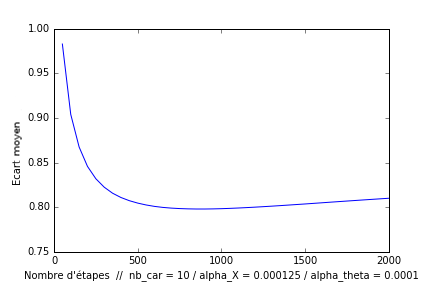
\includegraphics[scale=0.5]{yassine.png}
\caption{Ecart moyen entre les notes prédites et la réalité en fonction du nombre d'étape du gradient avec $n = 10$, $\alpha_X = 0.000125$ et $\alpha_\Theta = 0.0001$}
\end{figure}

\newpage

\section*{Conclusion}

Finalement, nous avons réussi à réaliser un programme qui, à partir d'un tableau de notes, 
peut prédire pour un certain nombre de films les notes d'utilisateurs quelconques ayant mis quelques notes. 
Cela avec une précision assez bonne : la moyenne des écarts absolus entre les notes prédites et la réalité vaut environ $0.79$. 
En tout cas, il s'agit d'une précision assez élevée pour pouvoir comparer des notes prédites pour 
un utilisateur et ainsi recommander le film ayant celle la plus élevée.\\

Améliorer encore notre système de recommandation ? Nous avons quelques idée à ce sujet.\\
D'abord utiliser une plus grande base de donnée : pour l'instant nous nous sommes limités à un peu plus de 9000 films mais nous pourrions largement augmenter ce nombre grâce aux donnée disponibles sur "movielens". Un plus grand nombre d'utilisateurs permettrait aussi une plus grande précision. Mais est un défi : une base de données trop grande rendrait notre algorithme très long à exécuter.\\
Autre chose, certaines méthodes existent pour limiter le sur-apprentissage sont nous avons parlé et que nous n'avons pas utilisée : le faire permettrait une précision plus élevée.\\
Développer une interface graphique pour notre système de recommandation serait aussi une chose intéressante : une application sur smartphone ou un site web rendrait facile d'utilisation notre système de recommandation et permettrait à beaucoup de personnes d'en profiter.\\
Enfin, nous avons décidé de prendre en compte seulement des notes d'utilisateurs pour nos prédictions. Mais d'autres données seraient utilisables comme le genre du film et la date à laquelle il a été noté. Il serait intéressant de se demander si cela augmenterait la précision de nos prédictions. Le genre du film serait sûrement peu intéressant puisque notre programme propose lui même les caractéristiques les mieux appropriés qu'il déduit des notes. Par contre, la date à laquelle a été noté le film pourrait bien augmenter la précision, référence \cite{matrix}.\\

Pour chacun de nous, ce projet fut passionnant et à apporté de nombreuses connaissances. Nous avons pu découvrir une partie du domaine de l'apprentissage automatique. Nous avons progressé au fur et à mesure de ce projet au niveau du travail en groupe. L'outil de travail collaboratif utilisé Github fut une découverte pour plusieurs d'entre nous et sera sûrement réutilisé par la suite. C'est aussi durant ce projet que certains ont appris à utiliser Latex, et cela nous sera aussi sûrement utile pour plus tard.\\
Pour toutes ces raisons ce projet nous a beaucoup apporté.

%Bibliographie 
\newpage 
 
\begin{thebibliography}{99} 
\bibitem{matrix} Matrix factorisation techniques for recommender systems, Y. Koren and R. Bell and C. Volinski ,IEEE Computer Society ,2009 ,pages 42-49 
\bibitem{mooc} MOOC - Machine Learning , Andrew Ng , Stanford University , date inconnue , Coursera.org
\end{thebibliography}

\newpage

\appendix
\section{Notations utilisés}
\label{notations}

Introduisons dans cette section les notations utilisés dans tout le rapport.\\ 

Nous travaillons tout au long de ce rapport avec des matrices réelles. $\forall (n, p) \in \mathbb{N}^2$ nous notons l'ensemble des matrices réelles de dimension $n * p$ : ${\cal M}_{n, p}$.\\ 
$\forall (n, p) \in \mathbb{N}^2$ $\forall A \in {\cal M}_{n, p}$ $\forall i \in \{1, 2, ..., n\}$ $a_i$ est la i-ème ligne de la matrice A et nous avons $a_i \in {\cal M}_{1, p}$. Et $\forall j \in \{1, 2, ..., p\}$ $a_{., j}$ est la j-ème colonne de la matrice A et nous avons $a_j \in {\cal M}_{n, 1}$. Remarquons que des majuscules sont utilisées pour des matrices qui ne sont ni des matrices lignes ni des matrices colonnes et des minuscules autrement. Nous utilisons aussi des minuscules pour les coefficients des matrices.\\ 
Sauf indication contraire, lorsque nous utilisons la lettre j il s'agit d'un entier naturel quelconque non nul et inférieur ou égal à $n_f$. De la même façon la lettre i représente, lorsque ça n'est pas précisé, un entier naturel quelconque non nul et inférieur ou égal à $n_u$.\\ 
Enfin, le film numéro j est le film dont les notes se trouvent à la j-ème colonne de Y et l'utilisateur i est l'utilisateur dont les notes qu'il a donné sont à la i-ème ligne de Y.\\

$||a|| = \sqrt{\sum_{k = 1}^{m} a_{k}^{2}}$ avec $m \in \mathbb{N}^*$ et $a \in {\cal M}_{m}$\\

Si $u$ est un vecteur de $\mathbb{R}^w$ avec $w \in \mathbb{N}^*$ et $f$ une fonction réelle dont une des variables est $u$ on a 
$\nabla_{u} f(u, ...) =
\begin{pmatrix}
\frac{\partial f}{\partial u_{1}}(u, ...)\\
\frac{\partial f}{\partial u_{2}}(u, ...)\\
\vdots\\
\frac{\partial f}{\partial u_{w}}(u, ...)
\end{pmatrix}$

\newpage

\section{Preuves}

\subsection{}  
\label{P1}
Les notations utilisées sont les mêmes que dans la partie 3.2. Montrons : \[\nabla_{(x_{j})^T} J(\Theta, X) = \nabla_{(x_{j})^T}\frac{1}{2}\Vert\tilde{\Theta}(x_{j})^{T}-\tilde{y}_{.,j}\Vert^{2}\]
Nous avons :
\begin{align*}
\nabla_{(x_{j})^T} J(\Theta, X) &=  
\begin{pmatrix}  
\displaystyle\frac{\partial \displaystyle\sum_{k=1}^{nf}\frac{1}{2}\Vert\tilde{\theta}(x_{k})^{T}-\tilde{y}_{.,k}\Vert^{2}}{\partial x_{j,1}}\\  
\displaystyle\frac{\partial \displaystyle\sum_{k=1}^{nf}\frac{1}{2}\Vert\tilde{\theta}(x_{k})^{T}-\tilde{y}_{.,k}\Vert^{2}}{\partial x_{j,2}}\\  
\vdots\\  
\displaystyle\frac{\partial \displaystyle\sum_{k=1}^{nf}\frac{1}{2}\Vert\tilde{\theta}(x_{k})^{T}-\tilde{y}_{.,k}\Vert^{2}}{\partial x_{j,n}}  
\end{pmatrix}  
=  
\begin{pmatrix}  
\displaystyle\sum_{k=1}^{nf}  
\frac{1}{2}\frac{\partial\Vert\tilde{\theta}(x_{k})^{T}-\tilde{y}_{.,k}\Vert^{2}}{\partial x_{j,1}}\\  
\displaystyle\sum_{k=1}^{nf}  
\frac{1}{2}\frac{\partial\Vert\tilde{\theta}(x_{k})^{T}-\tilde{y}_{.,k}\Vert^{2}}{\partial x_{j,2}}\\  
\vdots\\  
\displaystyle\sum_{k=1}^{nf}  
\frac{1}{2}\frac{\partial\Vert\tilde{\theta}(x_{k})^{T}-\tilde{y}_{.,k}\Vert^{2}}{\partial x_{j,n}}  
\end{pmatrix}\\
&=  
\begin{pmatrix}  
\displaystyle  
\frac{1}{2}\frac{\partial\Vert\tilde{\theta}(x_{j})^{T}-\tilde{y}_{.,j}\Vert^{2}}{\partial x_{j,1}}\\  
\displaystyle  
\frac{1}{2}\frac{\partial\Vert\tilde{\theta}(x_{j})^{T}-\tilde{y}_{.,j}\Vert^{2}}{\partial x_{j,2}}\\  
\vdots\\  
\displaystyle  
\frac{1}{2}\frac{\partial\Vert\tilde{\theta}(x_{j})^{T}-\tilde{y}_{.,j}\Vert^{2}}{\partial x_{j,n}}  
\end{pmatrix}
=  
\displaystyle  
\nabla_{(x_{j})^T}\frac{1}{2}\Vert\tilde{\Theta}(x_{j})^{T}-\tilde{y}_{.,j}\Vert^{2}
\end{align*}\\

Nous montrons de la même manière que : \[\nabla_{(\theta_{i})^T} J(\Theta, X) = \nabla_{(\theta_{i})^T}\frac{1}{2}\Vert\tilde{X}(\theta_{i})^{T}-\tilde{y}_{i}\Vert^{2}\]
\subsection{}  
\label{P2}
Montrons que $\forall n \in \mathbb{N}^{*}$ $\forall p \in \mathbb{N}^{*}$ si A est une matrice de dimension $p \times n$, x une matrice colonne de dimension $n \times 1$ et b une matrice colonne de dimension $p \times 1$ alors : \[\nabla_{x}\frac{1}{2}\Vert Ax-b \Vert^2 = A^{T}(Ax-b)\]
Soit $(n,p) \in (\mathbb{N}^*)^2$. Soient $A \in {\cal M}_{p, n}$, $x \in {\cal M}_{n, 1}$ et $b \in {\cal M}_{p, 1}$.\\
Pour montrer notre égalité, montrons que $\forall j \in \{1, 2, ..., p\}$ : \[[\nabla_{x} \frac{1}{2}||Ax - b||^{2}_{2}]_{j} = [A^{T}(Ax - b)]_{j}\]
Soit $j \in \{1, 2, ..., p\}$.
\begin{align*}  
[\nabla_{x} \frac{1}{2}||Ax - b||^{2}_{2}]_{j} &= [\nabla_{x} \frac{1}{2}(\sum^{n}_{i = 1} (\sum^{p}_{k = 1} A_{i, k}x_{k})^{2} - 2b_{i}(\sum^{p}_{k = 1} A_{i, k}x_{k}) + b_{i}^{2})]_{j}\\  
[\nabla_{x} \frac{1}{2}||Ax - b||^{2}_{2}]_{j} &= \frac{\partial\frac{1}{2}(\sum^{n}_{i = 1} (\sum^{p}_{k = 1} A_{i, k}x_{k})^{2} - 2b_{i}(\sum^{p}_{k = 1} A_{i, k}x_{k}) + b_{i}^{2})}{\partial x_{j}}\\  
[\nabla_{x} \frac{1}{2}||Ax - b||^{2}_{2}]_{j} &= \frac{1}{2}(\sum^{n}_{i = 1} 2(\sum^{p}_{k = 1} A_{i, k}x_{k})A_{i, j} - 2b_{i} A_{i, j})\\  
[\nabla_{x} \frac{1}{2}||Ax - b||^{2}_{2}]_{j} &= (\sum^{n}_{i = 1} (\sum^{p}_{k = 1} A_{i, k}x_{k})A_{i, j} - b_{i} A_{i, j})\\  
[\nabla_{x} \frac{1}{2}||Ax - b||^{2}_{2}]_{j} &= (\sum^{n}_{i = 1} A_{i, j}(\sum^{p}_{k = 1} A_{i, k}x_{k}) - b_{i} )\\  
[\nabla_{x} \frac{1}{2}||Ax - b||^{2}_{2}]_{j} &= \sum^{n}_{i = 1} A^{T}_{j, i}[Ax - b]_{i}\\  
[\nabla_{x} \frac{1}{2}||Ax - b||^{2}_{2}]_{j} &= [A^{T}(Ax - b)]_{j}  
\end{align*}

\newpage

\section{En pratique : recommandation d'un film à un nouvel utilisateur}
\label{specifique}

Au final une question intéressante est est-ce que le modèle arrivera d'une manière efficace à prédire les notes d'un nouvel utilisateur ?\\

Pour mettre en place cela nous choisissons de ne pas recalculer $X$ et $\Theta$ pour chaque nouvel utilisateur. À la place, nous supposons que l'ajout des notes d'un nouvel utilisateur ne va pratiquement pas modifier le calcul de $X$ et des profils des anciens utilisateurs. Il nous suffit donc de calculer et d'ajouter seulement une nouvelle ligne à $\Theta$, caractérisant le profil du nouvel utilisateur. Ceci peut alors se faire très rapidement. À partir de ces nouvelles données, il nous suffit de compléter la ligne de Y correspondant aux notes du nouvel utilisateur pour trouver la plus élevée et recommander à l'utilisateur le film associé.

\newpage

\section{Familiarisation avec problème plus simple}
\label{extrait}

Parlons d'un un autre problème plus simple, toujours dans le cadre de la recommandation de film grâce à la descente du gradient. Tout cela afin de bien comprendre comment fonctionne la descente du gradient.\\

Énonçons le problème. Comment, à partir d'un tableau de note qui ne contient qu'un seul NaN, prédire la note manquante sans factorisation de matrice ? Il faut imaginer un tableau de la même forme que Y auquel il manque une seul note tout en bas à droite. Un seul utilisateur n'a alors pas noté tous les films. Mais nous arrivons à un obstacle : où trouver ce tableau ?\\

Le problème qui se pose alors est de réussir à extraire de Y un sous-tableau plein auquel nous retirerons une note. Pour que notre travail soit assez intéressant, nous voulons que ce tableau soit le plus grand possible. En effet, avoir un grand tableau permettra de fournir plus de données à l'algorithme que nous créerons le rendant plus efficace. Nous cherchons alors à coder une fonction permettant d'extraire le plus grand tableau plein possible de Y. Or, il s'avère rapidement que cela est pratiquement impossible à faire et nous prend trop de temps. C'est pourquoi nous nous contentons de faire un algorithme renvoyant non pas le tableau extrait optimal, mais un tableau raisonnablement grand dont nous pouvons nous contenter. La matrice obtenue est $T \in {\cal M}_{u, f}$ avec $u = 25$ le nombre d'utilisateur et $f = 11$ le nombre de films. Le tableau est organisé de la même façon que Y et $t_{u, f} = NaN$ : seul l'utilisateur $u$ n'a pas noté le film $f$. Nous pouvons maintenant commencer à travailler. Nous oublions Y pour cette partie.\\

Notre méthode ? Réussir à trouver $f-1$ coefficients $a_1, a_2, ..., a_{f-1}$ tels que $\forall i \in \{1, 2, ..., u-1\}$ $t_{i, f} = \sum_{k = 1}^{f-1} a_k * t_{i, k}$, en supposant qu'ils existent. Alors il suffirait de prédire $t_{u, f}$ en supposant qu'il vaut $\sum_{k = 1}^{f-1} a_k * t_{u, k}$. Autrement dit, nous supposons qu'il existe la même relation linéaire pour chaque utilisateur entre les notes données par un utilisateur aux $f- 1$ premiers films et la note donnée par cet utilisateur au film f. Et nous essayons de déterminer cette relation.\\

Comment faire ? Notre but est de minimiser la fonction
\begin{align*}
\mathbb{R}^{f-1}&\longrightarrow \mathbb{R}^+\\ 
(a_1, a_2, ..., a_{f-1})&\longmapsto \frac{1}{2}\sum_{i = 1}^{u - 1} (\sum_{k = 1}^{f-1} (a_k * t_{i, k}) - t_{i, f})^2
\end{align*}
Tiens donc, minimiser une fonction ? Nous savons faire grâce à la descente du gradient. Et nous le faisons.\\

Maintenant nous pouvons nous demander à quel point cette méthode est précise. Nous utilisons donc notre algorithme sur plusieurs configurations du tableau T en enlevant à chaque fois une note différente du tableau extrait. Et nous observons un écart absolu moyen de 0.24 entre la note prédite et la valeur réelle de la note enlevée. Nous avons donc une très bonne précision sachant que les notes sont précises à 0.5 près. Mais malheureusement cette méthode ne peut être employée que sur un tableau qui n'a qu'une seule case vide.

\newpage

\section{Code} 
 
Dans cet annexe figure notre code. 
 
\subsection{Extraction des données et fonctions permettant leur manipulation, movielens.py} 
\begin{changemargin}{-4cm}{0cm} 
\lstinputlisting{movielens.py} 
\end{changemargin} 
 
\subsection{Statistiques sur nos données, stat.py} 
\begin{changemargin}{-4cm}{0cm} 
\lstinputlisting{stat.py} 
\end{changemargin} 
 
\subsection{Descente du gradient sur un tableau avec une seule note manquante, descente\_du\_gradient.py} 
\begin{changemargin}{-4cm}{0cm} 
\lstinputlisting{descente_du_gradient.py} 
\end{changemargin} 
 
\subsection{Prédiction des notes, recomendation\_system\_final.py} 
\begin{changemargin}{-4cm}{0cm} 
\lstinputlisting{recomendation_system_final.py} 
\end{changemargin} 
 
\subsection{Recherche des meilleurs paramètres, etude\_efficacite.py} 
\begin{changemargin}{-4cm}{0cm} 
\lstinputlisting{etude_efficacite.py} 
\end{changemargin}

\newpage

\vspace*{\stretch{1}}
\hrule height 1pt
\begin{center}
\begin{Large}Résumé\end{Large}
\end{center}
\hrule height 1pt
\vskip 1cm

La recommandation automatique est un domaine très intéressant qui peut susciter de la curiosité. Nous nous sommes intéressés à la recommandation 
automatique de film avec pour but de construire un programme pouvant recommander de manière personnalisée un film pertinent à n'importe quel utilisateur. Notre méthode s'appuie  
sur la factorisation de matrice, et la descente du gradient.\\ \\ \\ \\ \\ \\ 
 
\textbf{{Mots clés:}} descente du gradient, factorisation de matrices, prédiction de notes de films, informatique, programmation

\vspace*{\stretch{1}}

\end{document}
